
\section{Experimental Setup}\label{sec:expSetup}
In this section, we present the setup in our experimental platform. We show the datasets in Section~\ref{sec:datasets} and hardware/software setup in Section~\ref{sec:hwswsetup}.

\subsection{Datasets}\label{sec:datasets}

\subsubsection{Real Dataset}

We use the real dataset (provided by a commercial large-scale search engine company) in the experiment. The real dataset includes two parts: web data and query log. The web data contains more than 10 million web documents. The query log contains around 1 million real queries\footnote{The data source, as well as more detailed statistics about the web data and query log, is omitted for double-blind review purpose.}.


\subsubsection{Synthetic Dataset}
We also generate synthetic dataset (allowing to vary different parameters, e.g., inverted list size) to understand the cases that Smart SSD can win.
Below we show a number of key parameters to system performance, and the way that the data is generated.
Unless otherwise stated, we explain the parameters with two inverted lists, and when varying one particular parameter, we fix all the rest parameters as defaults.


\textbf{Number of lists}. By default, we evaluate the list operations (e.g., intersection) with two inverted lists: list \emph{A} and list \emph{B}. To capture the real cases that the list size is skewed (i.e., one list is longer than the other0, unless otherwise stated, we use list $A$ to indicate the shorter list while list $B$ the longer one in this paper. As we explained later, the size ratio between list $A$ and $B$ is determined by the \emph{skewness factor}. When varying the number of lists according to a parameter $m$ ($m>1$), we generate $m$ lists independently. Among them, half ($\lceil m/2\rceil$) of the lists are of the same size with list $A$ (i.e., shorter lists); another half ($\lfloor m/2\rfloor$) are of the same size with list $B$ (i.e., longer lists). We vary the number of lists from 2 to 8.

\textbf{List size skewness factor}. The \emph{skewness factor} (of list $A$ size and $B$ size) is defined as the ratio between the longer list size and shorter list size, i.e., $\frac{|B|}{|A|}$. In practice, the sizes of different lists differ a lot, because some query terms can be much more popular than the others. We set the skewness factor to be 100 and vary the skewness factor from 1 to 1000 to capture the real case\footnote{We randomly pick up 10,000 queries from the real query log and run them on the real web data. For each query, we record the skewness factor for the inverted lists involved. The average skewness factor is 3672. Even if we remove the top 20\% highest ones, it becomes 75.}.



\textbf{Intersection ratio}. The intersection ratio is defined as the intersection size over the shorter list, i.e., $\frac{|A\cap B|}{|A|}$ for two lists $A$ and $B$. By default, we set it to 1\% to reflect the real scenario. E.g., in Bing search, for 76\% of the queries, the intersection size is two orders of magnitude smaller than the shortest inverted list~\cite{Ding2011}. We vary the intersection ratio from 1\% to 100\%.


\textbf{List size}. Unless otherwise stated, the list size means the size of the \emph{longer} list, i.e., list \emph{B}.
By default, the size of list $B$ is 10MB\footnote{In real search engines, although the entire inverted index is huge, there are also a huge number of terms, thus, on average, each inverted list will not be very long (usually, 10s of MBs).}, and vary from 1MB to 100MB. The size of list $A$ can be obtained with the skewness factor. When the list size is determined, we randomly generate a list of entries (each includes document ID, score, and positional info) from a universe~\cite{Ding2011}.


Table~\ref{tab:synData} shows a summary of the key parameters, with defaults highlighted in bold.

\begin{table}[tbp]
\centering
\begin{tabular}{l|l}\hline\hline
\textbf{Parameters}  &   \textbf{Ranges}   \\\hline
Number of lists & \textbf{2}, 3, 4, 5, 6, 7, 8\\\hline
List size skewness factor  & 10000, 1000, \textbf{100}, 10, 1\\\hline
Intersection ratio  &   0.1\%, \textbf{1\%}, 10\%, 100\%\\\hline
List size & 1 MB, \textbf{10 MB}, 50 MB, 100 MB\\\hline\hline
\end{tabular}
\caption{Parameter setup}\label{tab:synData}
\end{table}






\subsection{Hardware and Software Setup}\label{sec:hwswsetup}
We carry out all the experiments in a commodity server with Intel i7 processor (3.40 GHz) and 8 GB memory, running Windows 7.
The Smart SSD is 400 GB SLC, connected to the server via a host bus adaptor (HBA) with 6Gbps. The regular SSD is the same SSD but with no offloaed application-specific code.


We measure the power consumption via the \emph{WattsUp}\footnote{\url{https://www.wattsupmeters.com}}.
Let $W_1$ and $W_2$ be the power (in Watts) when the system is idle and running, and $t$ be the query latency, then the energy is obtained by: $(W_2-W_1)\times t$.
\section{Experimental Results}\label{sec:expResults}

In this section, we present the results of offloading different query operations in Table~\ref{tab:designSpace}: \textsf{intersection} (Section~\ref{sec:expIntersection}), \textsf{ranked intersection} (Section~\ref{sec:expRankedIntersection}),
\textsf{difference} (Section~\ref{sec:expDifference}), \textsf{ranked difference} (Section~\ref{sec:expRankedDifference}), and \textsf{ranked union} (Section~\ref{sec:expRankedUnion}).

As explained in Section~\ref{sec:implementation}, we improved the original Lucene implementations on some list operations (e.g., intersection). Thus, we compare the following three approaches. (1) \emph{Smart SSD}: run our integrated Lucene and Smart SSD; (2) \emph{Regular SSD}: run the original Lucene on a regular SSD; (3) \emph{Regular SSD (optimized)}: run our optimized Lucene on a regular SSD.

We measure the average query latency and energy consumption. %We may also report the normalized values~\cite{Ding2011}.

\subsection{Intersection}\label{sec:expIntersection}
In this case, we offload the \textsf{intersection} (i.e., step X3 and X4 in Figure~\ref{fig:SmartSSDLucene}) to Smart SSD, while the ranking is done at the host side.


\stitle{Real data}
Table~\ref{tab:interRealData} shows the averaged query latency and energy consumed by a reply of real queries on real web data. It clearly shows that, compared to regular SSD, Smart SSD can reduce query latency by 3.6$\times$, and reduce energy by 10.4$\times$. Compared to the optimized regular SSD, Smart SSD still has a speedup of 2.2$\times$ in query latency and 6.7$\times$ in energy consumption.

The query latency saving comes from the high internal bandwidth and low I/O latency of Smart SSD. And the energy saving comes from less data movement and power-efficient processors (typically ARM series) running inside SSD.

\begin{table}[tbp]\small
\centering
\begin{tabular}{l|c|c}\hline\hline
& \textbf{Query latency (ms)} & \textbf{Energy (mJ)}\\\hline
Smart SSD & 97 & 204\\\hline
Regular SSD & 349 & 2129\\\hline
Regular SSD (optimized) & 210 & 1365 \\\hline\hline
\end{tabular}
\caption{Intersection on real data}\label{tab:interRealData}
\end{table}

\stitle{Effect of varying list size} Figure~\ref{fig:varyListSizeIntersection} evaluates the effect of different list sizes. We vary the size of list $B$ from 1MB to 100MB (while the size of list $A$ depends on the skewness factor, which is 100 by default). Both latency and energy increase with longer lists, because of more I/Os. But in any case, Smart SSD wins a lot. On average, Smart SSD improves performance by a factor of 3.5 while reduces energy by a factor of 10.5 compared to regular SSD. The two numbers are 2.5 and 7.8 compared to optimized regular SSD.


\begin{figure}[tbp]
  \centering
    \begin{tabular}{ccc}
 \includegraphics[width=0.95\columnwidth]{figures/banner.pdf}
\end{tabular}
\renewcommand{\tabcolsep}{0.1mm}
  \begin{tabular}{ccc}
 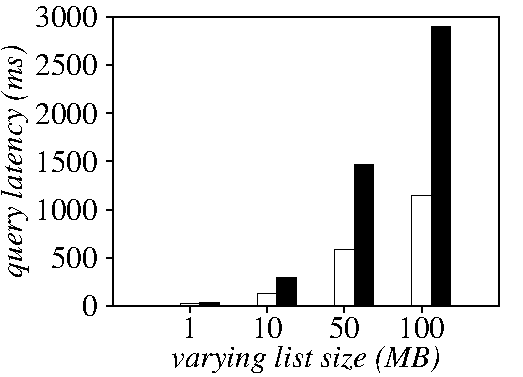
\includegraphics[width=0.5\columnwidth]{figures/Intersection-time-VaryListLen-eps-converted-to.pdf}&
  \includegraphics[width=0.5\columnwidth]{figures/Intersection-energy-VaryListLen-eps-converted-to.pdf}\\
  (a) query latency & (b) energy
\end{tabular}
  \caption{Varying the list size (for intersection)}
  \label{fig:varyListSizeIntersection}
 \end{figure}

\stitle{Effect of varying list size skewness factor}
Figure~\ref{fig:varyListSkewIntersection} shows the effect of list size skewness factor $f$, which can impact the intersection algorithm.
Higher skewness gives more chance for skipping data.
As the results of regular SSD are much worse than the other two approaches, for clear presentation, we show them separately in Figure~\ref{fig:varyListSkewIntersection}(c) and~\ref{fig:varyListSkewIntersection}(d). We fix the size of list $B$ to be 10MB, and vary the size of list $A$. The query latency (as well as energy) goes down when the skewness factor becomes higher. Because the size of list $A$ is becoming smaller. But in any case, Smart SSD wins.


\begin{figure}[htbp]
  \centering
    \begin{tabular}{ccc}
 \includegraphics[width=0.95\columnwidth]{figures/banner.pdf}%banner2.pdf
\end{tabular}
\renewcommand{\tabcolsep}{0.1mm}


  \begin{tabular}{ccc}
 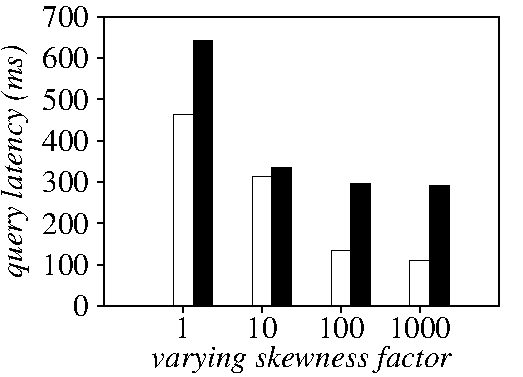
\includegraphics[width=0.5\columnwidth]{figures/Intersection-time-VaryListSkew2-eps-converted-to.pdf}&
  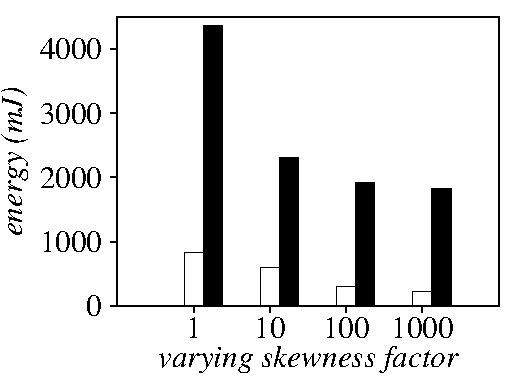
\includegraphics[width=0.5\columnwidth]{figures/Intersection-energy-VaryListSkew2-eps-converted-to.pdf}\\
  (a) query latency & (b) energy\\

  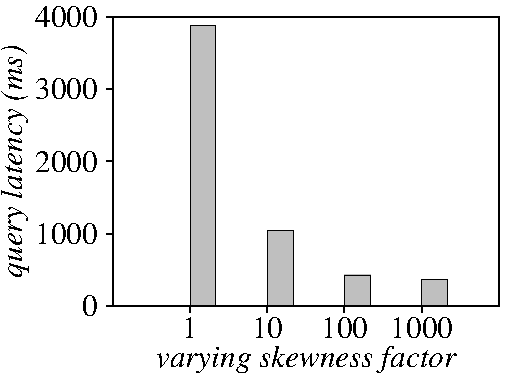
\includegraphics[width=0.5\columnwidth]{figures/Intersection-time-VaryListSkew1-eps-converted-to.pdf}&
  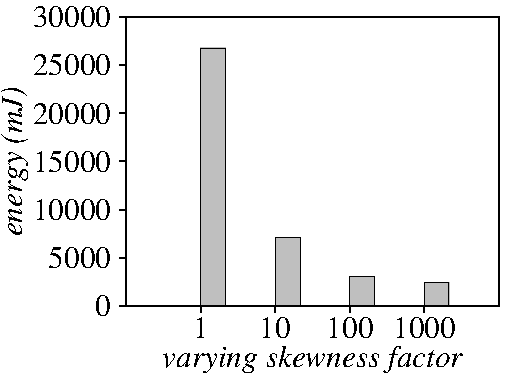
\includegraphics[width=0.5\columnwidth]{figures/Intersection-energy-VaryListSkew1-eps-converted-to.pdf}\\
  (c) query latency & (d) energy\\
\end{tabular}

  \caption{Varying the list size skewness factor (for intersection)}
  \label{fig:varyListSkewIntersection}
 \end{figure}


Besides the superiority of Smart SSD shown in Figure~\ref{fig:varyListSkewIntersection}, there are a number of interesting results. (1) When $f=1000$, the latency speedup achieves the largest (which is 2.6$\times$). That is because the sizes of the two lists different so much, which allows more data skipping using the adaptive intersection algorithm. The average number of memory accesses per page is 68. (2) When $f=1$, the latency speedup (1.4$\times$) is smaller than that when $f=1000$. That is because, in this case, the sort-merge algorithm is used, which scans the entire lists, without any skipping. The average number of memory accesses per page is 383. (3) When $f = 10$, the latency speedup (1.06$\times$) is the smallest. That is because the number of memory accesses per page (it is 640) is higher than the others\footnote{\scriptsize We analyze the reason why it is that high by estimating the number of memory accesses per page. Let $n_1$ and $n_2$ be the number of entries of list $A$ and $B$, then the total number of memory accesses using the adaptive intersection algorithm is roughly estimated as $n_1\cdot\log n_2$. Let $n_p$ be the total number of pages required, then the average number of memory accesses per page is $n_1\cdot\log n_2/n_p$. In this case, $n_1=(1MB/8 KB)*256=32768$, $n_2=(10MB/8KB)*256=327680$, $n_p=(1MB+10MB)/8KB=1408$. So, $n_1\cdot\log n_2/n_p=426$ (underestimated as binary search takes more than $\log n$ memory accesses.}. (4) When $f=1$, why regular SSD's performance is that bad (Figure~\ref{fig:varyListSkewIntersection}(c))? That is because of Lucene's implementation of list intersection. We find that, it is mostly because of invoking the \texttt{doNext()} function, see Figure~\ref{fig:doNext}. We take a time breakdown. Among the total 3877 ms, Line 2 takes around 814 ms, Line 3 takes 861 ms, Line 4--6 takes 1400 ms. The rest major cost is I/O, taking 550 ms (2564 pages). Note that, as the result size is small (3367), the ranking cost is negligible.

\begin{figure}[tbp]
	\centering
		\includegraphics[width=1\columnwidth]{figures/doNext.pdf}
	\caption{\small doNext() in /src/core/CLucene/search/ConjunctionScorer.cpp}
	\label{fig:doNext}
\end{figure}


\stitle{Effect of varying intersection ratio}
The intersection ratio determines the result size, which can impact system performance in two aspects: (1) data movement; and (2) ranking cost, which is required for each qualified document in the result set.

\begin{figure}[tbp]
\centering
\begin{tabular}{ccc}
\includegraphics[width=0.95\columnwidth]{figures/banner.pdf}
\end{tabular}
\renewcommand{\tabcolsep}{0.1mm}
\begin{tabular}{ccc}
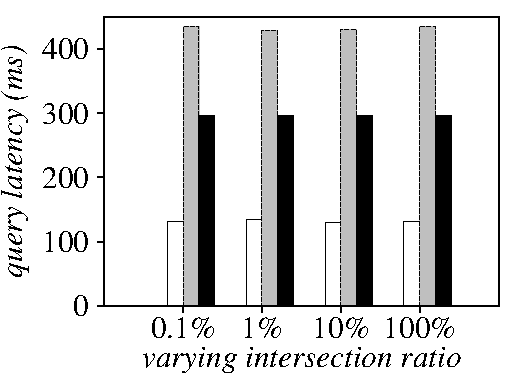
\includegraphics[width=0.5\columnwidth]{figures/Intersection-time-VaryInterRatio-eps-converted-to.pdf}&
\includegraphics[width=0.5\columnwidth]{figures/Intersection-energy-VaryInterRatio-eps-converted-to.pdf}\\
(a) query latency & (b) energy
\end{tabular}
\caption{Varying intersection ratio (for intersection)}
\label{fig:varyInterRatioIntersection1}
\end{figure}

Figure~\ref{fig:varyInterRatioIntersection1} shows impact of intersection ratio in the default case. Surprisingly, it does not show a clear impact. The reason is that, the skewness factor is 100, i.e., the size of list $A$ is 1\% smaller than list $B$. In this case, the maximum result size is 3367 (where the intersection ratio is 100\%), i.e., (3367 * 16bytes)/8KB = 7 pages = 1.4 ms, while the ranking cost is around 0.5 ms.



  \begin{figure}[tbp]
  \centering
    \begin{tabular}{ccc}
 \includegraphics[width=0.95\columnwidth]{figures/banner.pdf}
\end{tabular}
\renewcommand{\tabcolsep}{0.1mm}
  \begin{tabular}{ccc}
 \includegraphics[width=0.5\columnwidth]{figures/Intersection-time-VaryInterRatio-equal2-eps-converted-to.pdf}&
  \includegraphics[width=0.5\columnwidth]{figures/Intersection-energy-VaryInterRatio-equal2-eps-converted-to.pdf}\\
  (a) query latency & (b) energy\\
   \includegraphics[width=0.5\columnwidth]{figures/Intersection-time-VaryInterRatio-equal1-eps-converted-to.pdf}&
  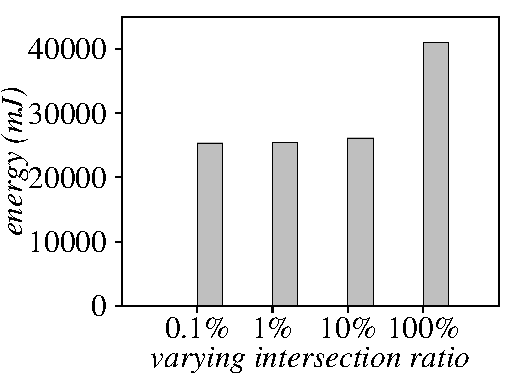
\includegraphics[width=0.5\columnwidth]{figures/Intersection-energy-VaryInterRatio-equal1-eps-converted-to.pdf}\\
  (c) query latency & (d) energy
\end{tabular}
  \caption{Varying intersection ratio on equal-sized lists (for intersection)}
  \label{fig:varyInterRatioIntersection2}
 \end{figure}


Then, we do the experiments again by setting the size of list $A$ to be the same as $B$, %The sizes are statistically the same, listA is 327668, listB is 327934, at 100\%, the intersection is 326918.
see Figure~\ref{fig:varyInterRatioIntersection2}. For clear presentation, we separated the results of regular SSD. We see a clear impact of intersection ratio (Figure~\ref{fig:varyInterRatioIntersection2}(a)). But in all cases, Smart SSD wins.
The query latency (as well as energy)  increases with higher intersection ratio, especially from intersection ratio 10\% to 100\%. For optimized regular SSD, the increase is because of the extra ranking cost. E.g., from 10\% to 100\%, the optimized regular SSD approach increase around 50 ms, because of dramatic intersection size increase from 32531 to 326918. For Smart SSD, the increase is because of two factors: more data transfer and ranking cost (at the host side). From 10\% to 100\%, the latency increased 163 ms. In which, data transfer increases around 110 ms (((326918 - 32531) * 16 / 8KB) * 0.2 = 115 ms), while the ranking cost increases around 50 ms, same as optimized regular SSD.



It is also interesting to see in Figure~\ref{fig:varyInterRatioIntersection2}, even when the intersection ratio is 100\%, Smart SSD can still win a bit over optimized regular SSD. That is because, in this case, Smart SSD only needs to transfer one list, saving around 50\% of data transfer.


%Besides that, it is also interesting to see that there is a latency jump between the intersection ratio 10\% and 100\% (Figure~\ref{fig:varyInterRatioIntersection2}(c)).  on regular SSD (lucene version): also a huge increase from 10\% to 100\% (around 2000 ms increase), one reason is because of ranking cost (800 ms more than 10\%), another reason is overhead in ConjunctionScorer::doNext(), where ``flag = more and first().doc smaller than last.doc()", taking around 1000 ms, because of more calls to doNext(), as cannot skip.


\stitle{Effect of varying number of lists}
Figure~\ref{fig:varyNumKeywordsIntersection} shows the results on the effect of varying the number of lists.
It clearly shows that executing intersection inside Smart SSD is much faster than on regular SSD (optimized).
The query latency (as well as energy) goes up with higher number of lists, because of more data transfer.
However, the performance is similar when the number of lists is 2 and 3 (similar for 4 and 5, 6 and 7).
That is because of the way we generate lists.
When the number of lists is 2, the generated two lists are $\{A, B\}$
When the number of lists is 3, the generated three lists are $\{A, B, A\}$.
Since list \emph{A} is 100$\times$ shorter than list \emph{B}, it will not incur much overhead in query latency.

  \begin{figure}[tbp]
  \centering
    \begin{tabular}{ccc}
 \includegraphics[width=0.95\columnwidth]{figures/banner.pdf}
\end{tabular}
\renewcommand{\tabcolsep}{0.1mm}
  \begin{tabular}{ccc}
 \includegraphics[width=0.5\columnwidth]{figures/Intersection-time-VaryNumLists-eps-converted-to.pdf}&
  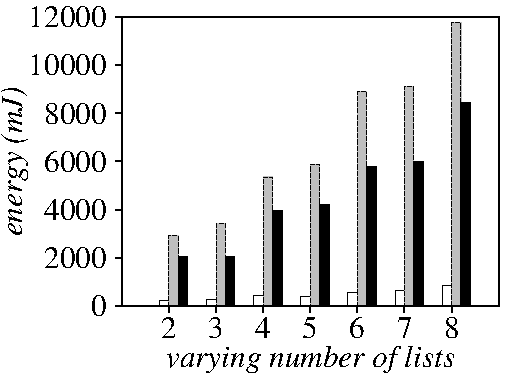
\includegraphics[width=0.5\columnwidth]{figures/Intersection-energy-VaryNumLists-eps-converted-to.pdf}\\
  (a) query latency & (b) energy
\end{tabular}
  \caption{Varying the number of lists (for intersection)}
  \label{fig:varyNumKeywordsIntersection}
 \end{figure}


\subsection{Ranked Intersection}\label{sec:expRankedIntersection}
In this case, we offload the \textsf{ranked intersection} (i.e., step X3, X4 and X5 in Figure~\ref{fig:SmartSSDLucene}) to Smart SSD. It will directly return results to host side. Compared to the offloading of intersection-only operation (Section~\ref{sec:expIntersection}), offloading ranked intersection can, (1) save more data transfer; but (2) increase the cost of ranking inside device. However, there is not much difference when the intersection result size is small (e.g., less than 30,000 entries, which is less than 5 ms).
Typically, the ranking cost is negligible, except when result size is very huge\footnote{As shown in Figure \protect\ref{fig:varyInterRatioIntersection2}, the ranking cost is around 50 ms when the intersection size is around 300,000.}.


\stitle{Real data}
Table~\ref{tab:rankInterRealData} shows the results by a replay of real queries on real web data. It shows that, Smart SSD  can reduce the query latency by a factor of 3.6 and 2.2 compared to regular SSD and optimized regular SSD, respectively. Besides that, Smart SSD can also reduce the energy by a factor of 13.2 and 7.8 compared to regular SSD and optimized regular SSD.

The results are similar to that in Table~\ref{tab:interRealData}. Because the average intersection size is 1144. Each entry takes 16 bytes (8-byte document ID and 8-byte score), i.e., 2 pages, which is around 0.4 ms. For regular SSD and optimized SSD, the I/O is also similar to that in Table~\ref{tab:interRealData}, as they have the same I/Os and ranking computation compared to the intersection-only offloading.

\begin{table}[tbp]\small
\centering
\begin{tabular}{l|c|c}\hline\hline
& \textbf{Query latency (ms)} & \textbf{Energy (mJ)}\\\hline
Smart SSD & 96 & 183\\\hline
Regular SSD & 351 & 2421\\\hline
Regular SSD (optimized) & 210 & 1428 \\\hline\hline
\end{tabular}
\caption{Ranked intersection on real data}\label{tab:rankInterRealData}
\end{table}

\stitle{Effect of varying list size}
The results are similar to the non-ranked version, i.e., Figure~\ref{fig:varyListSizeIntersection}. That is because the intersection result size does not differ that much. E.g., the maximum intersection size is 359 (when the list size is 100 MB) and the minimum intersection size is 3 (when the list size is 1 MB). Again, Smart SSD wins.


\stitle{Effect of varying list size skewness factor}
The results are similar to the non-ranked version, i.e., Figure~\ref{fig:varyListSkewIntersection}, because the intersection size is not that large. E.g., the maximum intersection size is 3877 (when the skewness factor is 1). Again, Smart SSD wins.

\stitle{Effect of varying intersection ratio}
The default case is similar to Figure~\ref{fig:varyInterRatioIntersection1}, where Smart SSD wins a lot. We show the results by setting the size of list $A$ to be the same as list $B$, see Figure~\ref{fig:varyRankInterRatioIntersection2}. The query latency (as well as energy) goes up with higher intersection ratio. However, it is interesting to see the increase is not that high compared to the results in Figure~\ref{fig:varyInterRatioIntersection2} for non-ranked intersection offloading. E.g., for Smart SSD, when the intersection ratio goes from 10\% to 100\%, the latency increases by 65 ms, while the corresponding increase in Figure~\ref{fig:varyInterRatioIntersection2} is 163ms. The increase does not go that much is because of no extra data movement (only top-$k$ results are returned), i.e., the increase is owing to the extra ranking cost (while the extra ranking cost at the host side is 50 ms).

It is also interesting to see from Figure~\ref{fig:varyRankInterRatioIntersection2} that, when the intersection ratio is 100\%, Smart SSD wins much more than the non-ranked version (Figure~\ref{fig:varyInterRatioIntersection2}). That is because of much less data movement as only top-$k$ results are returned.


  \begin{figure}[tbp]
  \centering
    \begin{tabular}{ccc}
 \includegraphics[width=0.95\columnwidth]{figures/banner.pdf}
\end{tabular}
\renewcommand{\tabcolsep}{0.1mm}
  \begin{tabular}{ccc}
 \includegraphics[width=0.5\columnwidth]{figures/RankIntersection-time-VaryInterRatio-equal2-eps-converted-to.pdf}&
  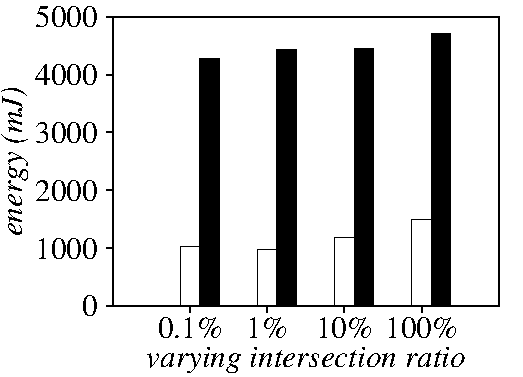
\includegraphics[width=0.5\columnwidth]{figures/RankIntersection-energy-VaryInterRatio-equal2-eps-converted-to.pdf}\\
  (a) query latency & (b) energy\\
   \includegraphics[width=0.5\columnwidth]{figures/RankIntersection-time-VaryInterRatio-equal1-eps-converted-to.pdf}&
  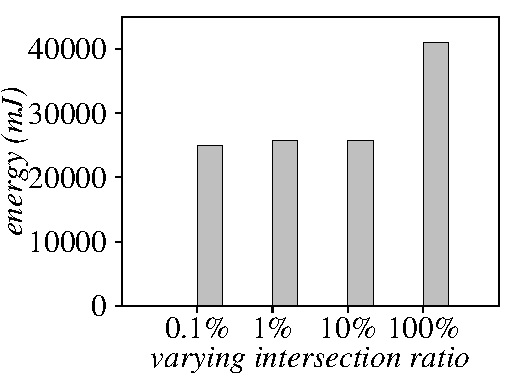
\includegraphics[width=0.5\columnwidth]{figures/RankIntersection-energy-VaryInterRatio-equal1-eps-converted-to.pdf}\\
  (c) query latency & (d) energy
\end{tabular}
  \caption{Varying intersection ratio on equal-sized lists (for ranked intersection)}
  \label{fig:varyRankInterRatioIntersection2}
 \end{figure}


\ntitle{Effect of varying number of lists}
The results are similar to the non-ranked version shown in Figure~\ref{fig:varyNumKeywordsIntersection} because the intersection size is very small (only 47), which will not make a major difference.

\subsection{Difference}\label{sec:expDifference}

In this case, we offload the \textsf{difference} operation (i.e., step X3 and X4 in Figure~\ref{fig:SmartSSDLucene}) to Smart SSD. The \textsf{difference} operator is usually applied to two lists, and is ordering-sensitive, it can be $(A-B)$ or $(B-A)$, where the list $A$ is shorter than list $B$. Intuitively, Smart SSD can benefit the former case (see Section~\ref{sec:designSpace}). The ranking is done at the host side. But ranking is very fast, as only need to consider one list.

\stitle{Real data}
Table~\ref{tab:diffRealData} shows the results by a replay of the real queries on the real web data. For each query, we consider the $(A-B)$ case, where $A$ and $B$ indicate the shortest and longest lists in a query. It clearly shows that, compared to the optimized regular SSD, Smart SSD can reduce the query latency and energy by a factor of 2.5 and 8.5, respectively. The gap is even larger if compared to regular SSD.

It is also interesting to note that, the performance of regular SSD (i.e., Lucene's original implementation) is only 13.4\% worse compared to the optimized regular SSD. That is because, there is no heap-adjustment involved as discussed in Section~\ref{sec:difference}.

\begin{table}[htbp]\small
\centering
\begin{tabular}{l|c|c}\hline\hline
& \textbf{Query latency (ms)} & \textbf{Energy (mJ)}\\\hline
Smart SSD & 78 & 148\\\hline
Regular SSD & 220 & 1430\\\hline
Regular SSD (optimized) & 194 & 1261 \\\hline\hline
\end{tabular}
\caption{Difference on real data}\label{tab:diffRealData}
\end{table}

\ntitle{Effect of varying list size}
Figure~\ref{fig:varyListSizeDifference} plots the effect of varying list sizes to the system performance.
The query latency (as well as energy) goes up with longer lists. But Smart SSD wins.

\begin{figure}[hbtp]
  \centering
    \begin{tabular}{ccc}
 \includegraphics[width=0.95\columnwidth]{figures/banner.pdf}
\end{tabular}
\renewcommand{\tabcolsep}{0.1mm}
  \begin{tabular}{ccc}
 \includegraphics[width=0.5\columnwidth]{figures/Difference-time-VaryListLen-eps-converted-to.pdf}&
  \includegraphics[width=0.5\columnwidth]{figures/Difference-energy-VaryListLen-eps-converted-to.pdf}\\
  (a) query latency & (b) energy
\end{tabular}
  \caption{Varying the list size (for difference)}
  \label{fig:varyListSizeDifference}
 \end{figure}




\stitle{Effect of varying list size skewness factor}
The skewness factor is a key factor in \textsf{difference} operation.
We consider $(A-B)$, but in this case, list $A$ is not necessarily smaller than $B$, depending on the skewness factor, which is still defined as $|B|/|A|$.
Figure~\ref{fig:varyListSkewDifference} plots the effect of skewness factor $f$, with the corresponding list sizes shown in Table~\ref{tab:skewFactorDifference}.


\begin{figure}[H]
  \centering
    \begin{tabular}{ccc}
 \includegraphics[width=0.95\columnwidth]{figures/banner.pdf}%banner2.pdf
\end{tabular}
\renewcommand{\tabcolsep}{0.1mm}


  \begin{tabular}{ccc}
 \includegraphics[width=0.5\columnwidth]{figures/Difference-time-VaryListSkew-eps-converted-to.pdf}&
  \includegraphics[width=0.5\columnwidth]{figures/Difference-energy-VaryListSkew-eps-converted-to.pdf}\\
  (a) query latency & (b) energy
\end{tabular}

  \caption{Varying the list size skewness factor (for difference)}
  \label{fig:varyListSkewDifference}
 \end{figure}


\begin{table}[htbp]\small
\centering
\begin{tabular}{l|l|l}\hline\hline
\textbf{Skewness factor} & \textbf{Size of list $A$} & \textbf{Size of list} $B$\\\hline
0.01 & 10 MB & 0.1 MB\\\hline
0.1 & 10 MB & 1 MB\\\hline
1 & 10 MB & 10 MB\\\hline
10 & 1 MB & 10 MB \\\hline
100 & 0.1 MB & 10 MB\\\hline\hline
\end{tabular}
\caption{Skewness factor and corresponding list sizes in Figure~\ref{fig:varyListSkewDifference}}\label{tab:skewFactorDifference}
\end{table}

Figure~\ref{fig:varyListSkewDifference} shows several interesting results. (1)Smart SSD loses in terms of query latency when the skewness factor $f=0.01$ and $f=0.1$ (compared to the optimized regular SSD). That is because, when $f=0.01$ or 0.1, the result size of $(A-B)$ does not save much data transfer. E.g., when $f=0.01$ the result size is 326437, which is almost the same as $|A| + |B|$. But Smart SSD can still reduce the energy due to power-efficient processors running inside SSD. (2) When $f$ goes from $0.01$ to $0.1$, for Smart SSD, why the query latency goes up? That is because of more memory access when $f=0.1$\footnote{\small In both cases where $f=0.01$ or $f=0.1$, $A$ is the same, i.e., 10 MB, see Table~\ref{tab:skewFactorDifference}. However, when $f=0.1$, $B$ is longer. While the total number of memory accesses can be roughly estimated as $|A|\cdot\log |B|$, thus, there is more memory access when $f=0.1$. In terms of the number of memory accesses per page, it is 3266 ($f=0.1$) and 2723 ($f=0.01$).}. (3) Why Smart SSD wins when $f=1$? That is because we can still reduce data transfer by 50\%. (4) Why Smart SSD wins at both $f=10$ and $f=100$? Much less data transfer. (5) For optimized regular SSD, why it reaches the highest latency when $f=1$? Because at this point, both of the lists are of 10 MB, which needs more data transfer. (6) Why the query performance is better when $f=10$ compared to $f=0.1$? Because of less memory access when $f=10$ (with the estimated equation: $|A|\cdot\log |B|$). (7) As a comparison, when $f=1$, both lists are of size 10 MB. This case is similar to Figure~\ref{fig:varyInterRatioIntersection2}(a) where the intersection ratio is 100\%. Because both are using sort-merge based algorithm, and can save around 50\% of data transfer. Thus, echo the results in~\ref{fig:varyInterRatioIntersection2}(a).


%1. Smart SSD loses at 0.01 and 0.1 point. at 0.01, A = 10 MB, B = 0.1MB, A-B does not save much, result size is 326437. at 0.1, A = 10MB, B = 1MB, A-B also does not save much, result size is 327790

%2. For Smart SSD, why worse at 0.1? Compare 0.01 and 0.1 points, both A = 10MB, but at 0.1 point, B is large. According to A*log B, meaning that, at 0.1 point, memory access more. Although at 0.1 point, total num of pages are a little more (1412 vs 1290), on avg, 0.1 point, avg mem access per page is higher (3266 vs 2723)

% 3. For Smart SSD, why win at 1 point? as two lists are of 10MB, in which case, save at least one list transfer

% 4. For Smart SSD, why win at 10 and 100? less data transfer

%5. For normal SSD, why it reaches the highest point at 1? as two lists are 10MB, more data transfer

%6. why 10 is less than 0.1? as 10*log (0.1) vs 0.1*log(10)

%7. Comparison: 10MB vs 10MB, i.e, at point skew 1. This case is similar to Fig 9a(100\% point). As, both are saving around one list. And, using sort-merge algo. Echo results!


\stitle{Effect of varying intersection ratio}
The intersection ratio is also a key factor, as higher intersection ratio means less common elements to transfer. For clear presentation, we set the size list $A$ to be the same as list $B$\footnote{As discussed before, there is no noticeable changes when the size of list $A$ is 1\% of list $B$.}, see Figure~\ref{fig:varyInterRatioDifference}.

\begin{figure}[tbp]
\centering
\begin{tabular}{ccc}
\includegraphics[width=0.95\columnwidth]{figures/banner.pdf}
\end{tabular}
\renewcommand{\tabcolsep}{0.1mm}
\begin{tabular}{ccc}
\includegraphics[width=0.5\columnwidth]{figures/Difference-time-VaryInterRatio-equal-eps-converted-to.pdf}&
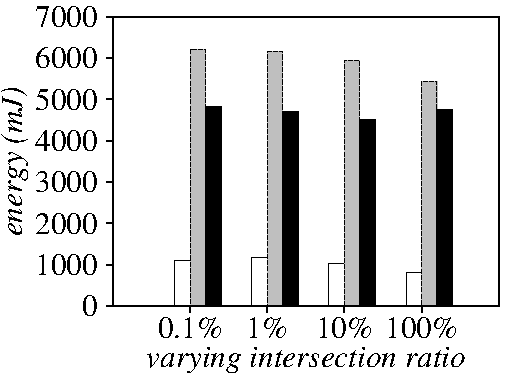
\includegraphics[width=0.5\columnwidth]{figures/Difference-energy-VaryInterRatio-equal-eps-converted-to.pdf}\\
(a) query latency & (b) energy
\end{tabular}
\caption{Varying intersection ratio (for difference)}
\label{fig:varyInterRatioDifference}
\end{figure}

Figure~\ref{fig:varyInterRatioDifference} shows that, for Smart SSD, the query latency generally goes down with higher intersection ratio, although not clear when the ratio is 0.1\%, 1\% and 10\% (due to the result size is similar). However, there is a clear latency drop at 100\% because of much less data transfer.
\subsection{Ranked Difference}\label{sec:expRankedDifference}
In this case, we offload the ranked difference (i.e., step X3, X4 and X5 in Figure~\ref{fig:SmartSSDLucene}).

\stitle{Real data}
See Table~\ref{tab:rankDiffRealData}, which is similar to Table~\ref{tab:diffRealData} as the average result size is small (3109 on average).

\begin{table}[tbp]\small
\centering
\begin{tabular}{l|c|c}\hline\hline
& \textbf{Query latency (ms)} & \textbf{Energy (mJ)}\\\hline
Smart SSD & 77  & 139\\\hline
Regular SSD & 201 & 1377\\\hline
Regular SSD (optimized) & 168 & 1109 \\\hline\hline
\end{tabular}
\caption{Ranked difference on real data}\label{tab:rankDiffRealData}
\end{table}

\stitle{Effect of varying list size}
Similar to non-ranked version, as result size is small (maximum is 32204).

\stitle{Effect of varying list size skewness factor}
The skewness factor determines the result size. For the non-ranked version (see Figure~\ref{fig:varyListSkewDifference}),
Smart SSD loses when $f=0.01$ and $f=0.1$, due to large result size.
Thus, with ranking function applied, the result size will be much smaller. Thus, we conjecture Smart SSD will win for all cases.

However, surprisingly, Smart SSD loses when $f=0.01$ and 0.1. That is because,
there are too many memory access at these two cases in order to get the results (estimated by $|A|\cdot\log |B|$), regardless of any data transfer.
The number of memory accesses per page is 1290 ($f=0.01$) and 1412 ($f=0.1$), respectively.

It is also interesting to see from Figure~\ref{fig:varyListSkewDifference} when $f=1$, the speedup of Smart SSD becomes larger (compared to Figure~\ref{fig:varyListSkewDifference}) due to less data transfer.

\begin{figure}[tbp]
  \centering
    \begin{tabular}{ccc}
 \includegraphics[width=0.95\columnwidth]{figures/banner.pdf}%banner2.pdf
\end{tabular}
\renewcommand{\tabcolsep}{0.1mm}


  \begin{tabular}{ccc}
 \includegraphics[width=0.5\columnwidth]{figures/RankDifference-time-VaryListSkew-eps-converted-to.pdf}&
  \includegraphics[width=0.5\columnwidth]{figures/RankDifference-energy-VaryListSkew-eps-converted-to.pdf}\\
  (a) query latency & (b) energy
\end{tabular}

  \caption{Varying the list size skewness factor (for ranked difference)}
  \label{fig:varyListSkewRankDifference}
 \end{figure}

%\textcolor{red}{Exp: should be different from non-ranked version. We will always win.} However, we lose! That is because the memory access it too many (in order to get the results)

%1. At 100 and 10, we win

%2. Why lose at 0.01 and 0.1? That's because in order to get the intersection results, we accessed too many memory! A*logB.

%3. Why still win at 1? (1) mem access is small as using sort-merge; (2) the gap is larger, as no need for data transfer.
% (3) save one list transfer. Actually, similar to Fig11a: Comparison: 10MB vs 10MB, i.e, at point skew 1.
% This case is similar to Fig11a(100\% point). As, both are saving around one list. And, using sort-merge algo.
% Echo results!

\stitle{Effect of varying intersection ratio}
Figure~\ref{fig:varyInterRatioRankDifference} shows the impact of varying intersection ratio to system performance.
It clearly shows the superiority of Smart SSD in terms of both query latency and energy.
It is interesting to see the latency speedup is larger when the intersection ratio is 0.1\%, 1\% and 10\% compared to Figure~\ref{fig:varyInterRatioDifference}, because of less data transfer after ranking. It is also interesting to see a slightly drop when the intersection ratio goes from 10\% to 100\%, because the result size is very small when at 100\%.

 \begin{figure}[tbp]
\centering
\begin{tabular}{ccc}
\includegraphics[width=0.95\columnwidth]{figures/banner.pdf}
\end{tabular}
\renewcommand{\tabcolsep}{0.1mm}
\begin{tabular}{ccc}
\includegraphics[width=0.5\columnwidth]{figures/RankDifference-time-VaryInterRatio-equal-eps-converted-to.pdf}&
\includegraphics[width=0.5\columnwidth]{figures/RankDifference-energy-VaryInterRatio-equal-eps-converted-to.pdf}\\
(a) query latency & (b) energy
\end{tabular}
\caption{Varying intersection ratio (for ranked difference)}
\label{fig:varyInterRatioRankDifference}
\end{figure}


\subsection{Ranked Union}\label{sec:expRankedUnion}
In this case, we offload the ranked union (i.e., step X3, X4 and X5 in Figure~\ref{fig:SmartSSDLucene}). We first present the results in Section~\ref{sec:rankUnionResults}, then discuss more on optimizations in Section~\ref{sec:rankUnionOpt}.

\subsubsection{Results}\label{sec:rankUnionResults}
\stitle{Real data}
Table~\ref{tab:unionRealData} shows the results on real data. It shows that, Smart SSD loses around 1.7$\times$ compared to the optimized regular SSD, in query latency. However, it reduces energy consumption by a factor of 2.1$\times$, because of power-efficient processors running inside SSD. The reason why Smart SSD loses is because of too many memory accesses. That is because, in practice, the union result set size is similar to the sum of each individual list size. Thus, every list has to be accessed $2k$ times, where $k$ is the number of keywords per query. On average, $k=3.8$ in our query log. Thus, all the lists have to be accessed approximately 7.6 times.
\begin{table}[htbp]\small
\centering
\begin{tabular}{l|c|c}\hline\hline
& \textbf{Query latency (ms)} & \textbf{Energy (mJ)}\\\hline
Smart SSD & 505 & 960 \\\hline
Regular SSD & 392 & 2704 \\\hline
Regular SSD (optimized) & 299 & 2033  \\\hline\hline
\end{tabular}
\caption{Ranked union on real data}\label{tab:unionRealData}
\end{table}


\stitle{Effect of varying intersection ratio}
The intersection ratio determines the result size.
Figure~\ref{fig:varyInterRatioRankUnion} evaluates the impact of intersection ratio to system performance, with two equal-sized lists (10 MB).
It shows, except when the intersection ratio is 100\%, Smart SSD loses around 1.2$\times$ in query latency. That is because, the result size is smaller than other cases, incurring less number of memory accesses.

\begin{figure}[tbp]
\centering
\begin{tabular}{ccc}
\includegraphics[width=0.95\columnwidth]{figures/banner.pdf}
\end{tabular}
\renewcommand{\tabcolsep}{0.1mm}
\begin{tabular}{ccc}
\includegraphics[width=0.5\columnwidth]{figures/RankUnion-time-VaryInterRatio-eps-converted-to.pdf}&
\includegraphics[width=0.5\columnwidth]{figures/RankUnion-energy-VaryInterRatio-eps-converted-to.pdf}\\
(a) query latency & (b) energy
\end{tabular}
\caption{Varying intersection ratio (for ranked union)}
\label{fig:varyInterRatioRankUnion}
\end{figure}


\stitle{Effect of varying list size skewness factor}
Figure~\ref{fig:varyListSkewRankUnion} shows the impact of the skewness factor. In all cases, Smart SSD loses around 1.2$\times$.

\begin{figure}[htbp]
  \centering
    \begin{tabular}{ccc}
 \includegraphics[width=0.95\columnwidth]{figures/banner.pdf}%banner2.pdf
\end{tabular}
\renewcommand{\tabcolsep}{0.1mm}


  \begin{tabular}{ccc}
 \includegraphics[width=0.5\columnwidth]{figures/RankUnion-time-VaryListSkew-eps-converted-to.pdf}&
  \includegraphics[width=0.5\columnwidth]{figures/RankUnion-energy-VaryListSkew-eps-converted-to.pdf}\\
  (a) query latency & (b) energy
\end{tabular}

  \caption{Varying the list size skewness factor (for ranked union)}
  \label{fig:varyListSkewRankUnion}
 \end{figure}


\stitle{Effect of varying list size}
Figure~\ref{fig:varyListLenRankUnion} shows the impact of list size. In all cases, Smart SSD loses around 1.2$\times$.

  \begin{figure}[htbp]
  \centering
    \begin{tabular}{ccc}
 \includegraphics[width=0.95\columnwidth]{figures/banner.pdf}
\end{tabular}
\renewcommand{\tabcolsep}{0.1mm}
  \begin{tabular}{ccc}
 \includegraphics[width=0.5\columnwidth]{figures/RankUnion-time-VaryListLen-eps-converted-to.pdf}&
  \includegraphics[width=0.5\columnwidth]{figures/RankUnion-energy-VaryListLen-eps-converted-to.pdf}\\
  (a) query latency & (b) energy
\end{tabular}
  \caption{Varying the list size (for ranked union)}
  \label{fig:varyListLenRankUnion}
 \end{figure}

  \begin{figure}[H]
  \centering
    \begin{tabular}{ccc}
 \includegraphics[width=0.95\columnwidth]{figures/banner.pdf}
\end{tabular}
\renewcommand{\tabcolsep}{0.1mm}
  \begin{tabular}{ccc}
 \includegraphics[width=0.5\columnwidth]{figures/RankUnion-time-VaryNumLists-eps-converted-to.pdf}&
  \includegraphics[width=0.5\columnwidth]{figures/RankUnion-energy-VaryNumLists-eps-converted-to.pdf}\\
  (a) query latency & (b) energy
\end{tabular}
  \caption{Varying the number of lists (for ranked union)}
  \label{fig:varyNumKeywordsRankUnion}
 \end{figure}
\stitle{Effect of varying number of lists}
Figure~\ref{fig:varyNumKeywordsRankUnion} shows the impact of number of lists $k$ in a query. It shows that, the gap between Smart SSD and regular SSD becomes larger with more number of lists. That is because, approximately, each list has to be accessed $2k$ times.



\subsubsection{Discussion: Call for Algorithmic Optimizations}\label{sec:rankUnionOpt}
The reason why it is not cost-effective to offload ranked union is because of too many memory accesses.
To improve the performance, on the one hand, we could improve the intrinsic performance of Smart SSD by improving memory access speed.
On the other hand, more efficient Smart SSD aware algorithms are to be designed. More importantly, one needs to be careful about the \emph{hidden constant} of algorithms, not only big O notation. E.g., the sort-merge based union algorithm is in linear cost, however, the hidden constant factor slows down the performance significantly.

\textbf{A special case of ranked union on \emph{two} lists.} If the number of lists is 2, a better algorithm for Smart SSD can be as follows. (1) Find the intersection results $R$ between $k$ lists $L_1, L_2, \cdots, L_k$. It takes, usually, less than 1 scan of all lists; (2) Scan Scan $R$, and $L_1, L_2, \cdots, L_k$ to find the top ranked results. It takes 1 scan. Thus, in total, around 2 full scans on all the $k$ lists. In this case, Samrt SSD wins. 
